\chapter{Supporting results for structural predictors}\label{appen:SuppPredictors}

%Here we add some details on the supporting results of  Chapter~\ref{chp:2}.

\section{Persistence not equal to 50\%} \label{SI:1}
\begin{figure}[h]
    \centering
    \includegraphics[width=\textwidth]{figures/appendices/fig_Importance_mut_persisNOT50.pdf}
    \caption[Importance profile when persistence is not $50\%$]{Normalized importance for empirical network $\texttt{Emp}$\_$\texttt{IL}$ ($N = 1500$) with only mutualistic interactions when persistence is $30\%$ ($\alpha_+ = 0.05$) and $80\%$ ($\alpha_+ = 0.03$).}
\end{figure}

\newpage
\section{Metrics over time} \label{SI:2}
\begin{figure}[h]
    \centering
    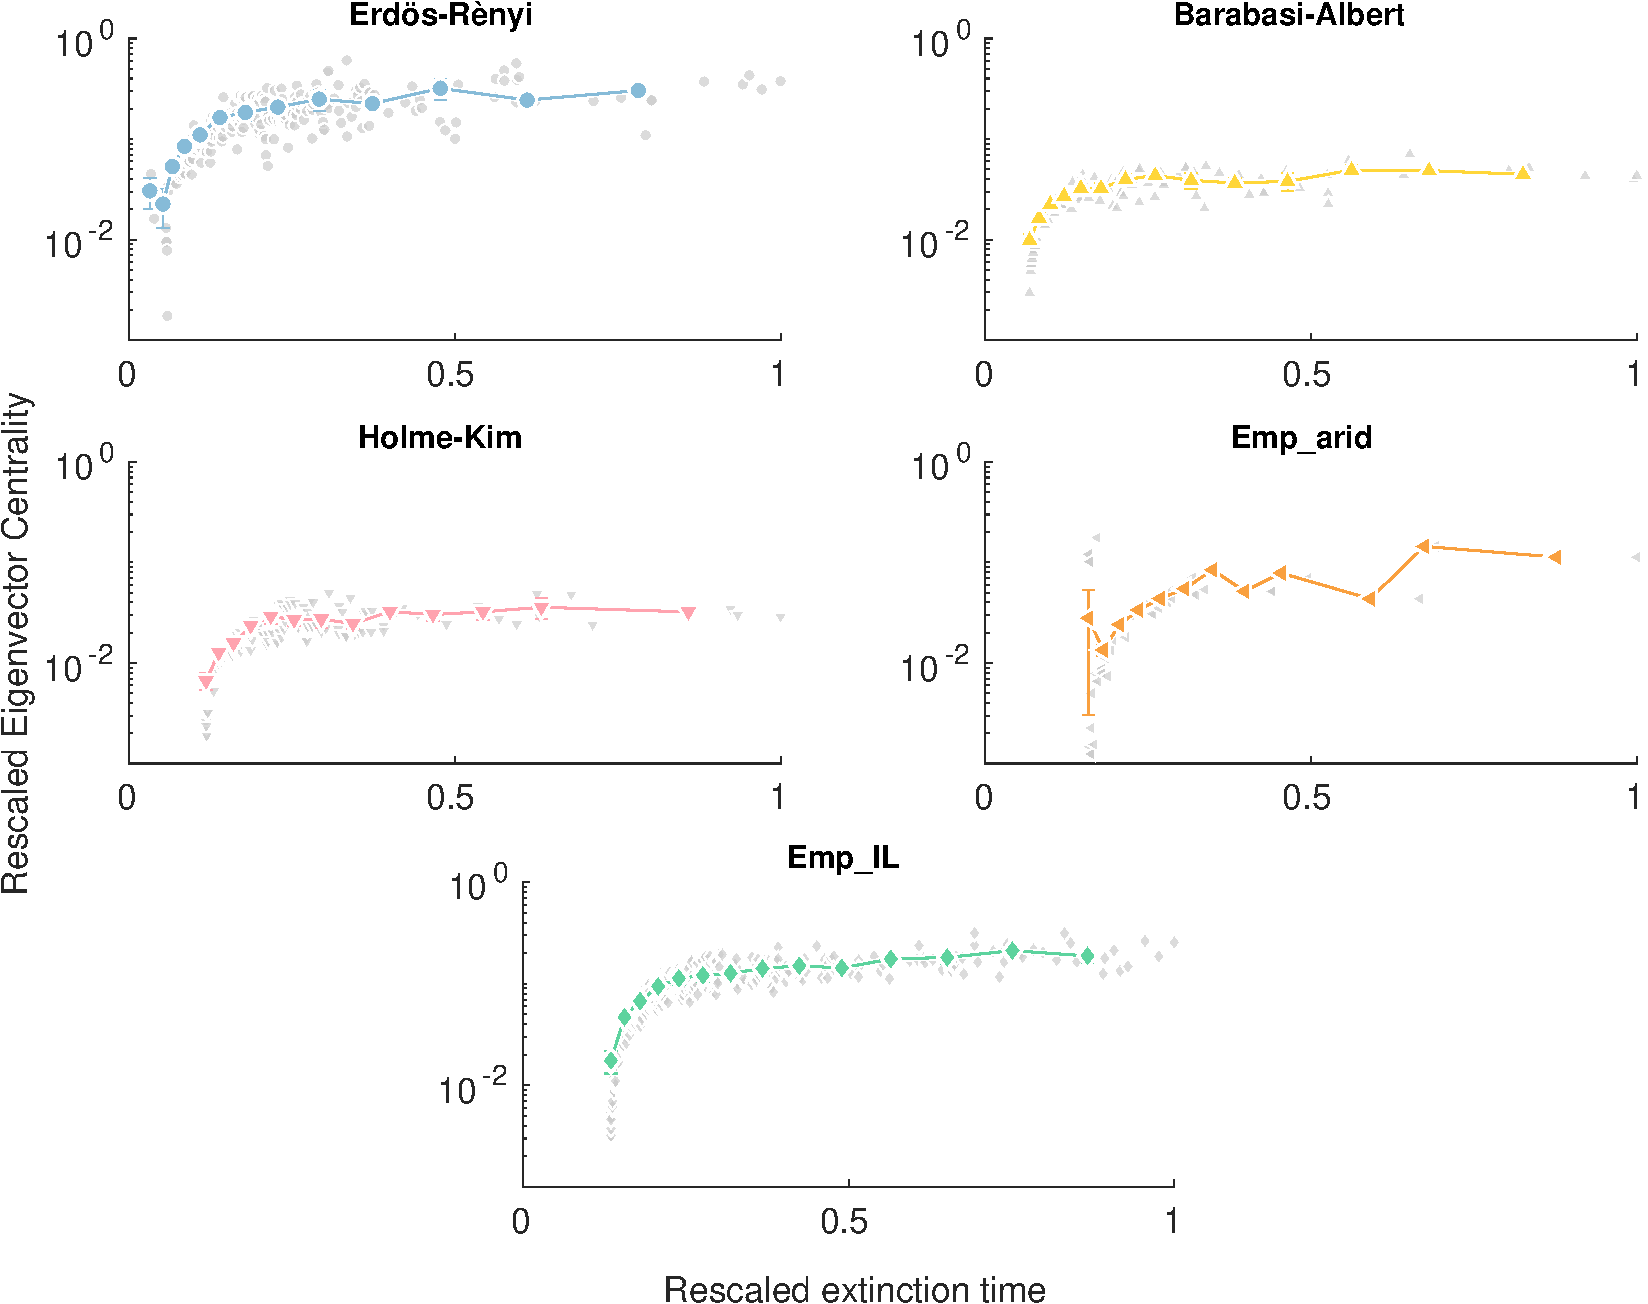
\includegraphics[width=\textwidth]{figures/chp2/figSI2_mut.pdf}
    \caption[Evolution of the eigenvector centrality of extinct species]{Eigenvector centrality of each species in function of the time it extinguishes in a mutualistic community for the different network models. These panels report the same data shown in Figure~\ref{chp2:fig:6}b. Each gray point is a species. Colored points are the average eigenvector centrality calculated over logarithmically spaced bins. Error bars (sometimes too short to be seen) denote the standard deviation from the mean.}
    \label{chp2:fig:SI2_mut}
\end{figure}

\begin{figure}[h]
    \centering
    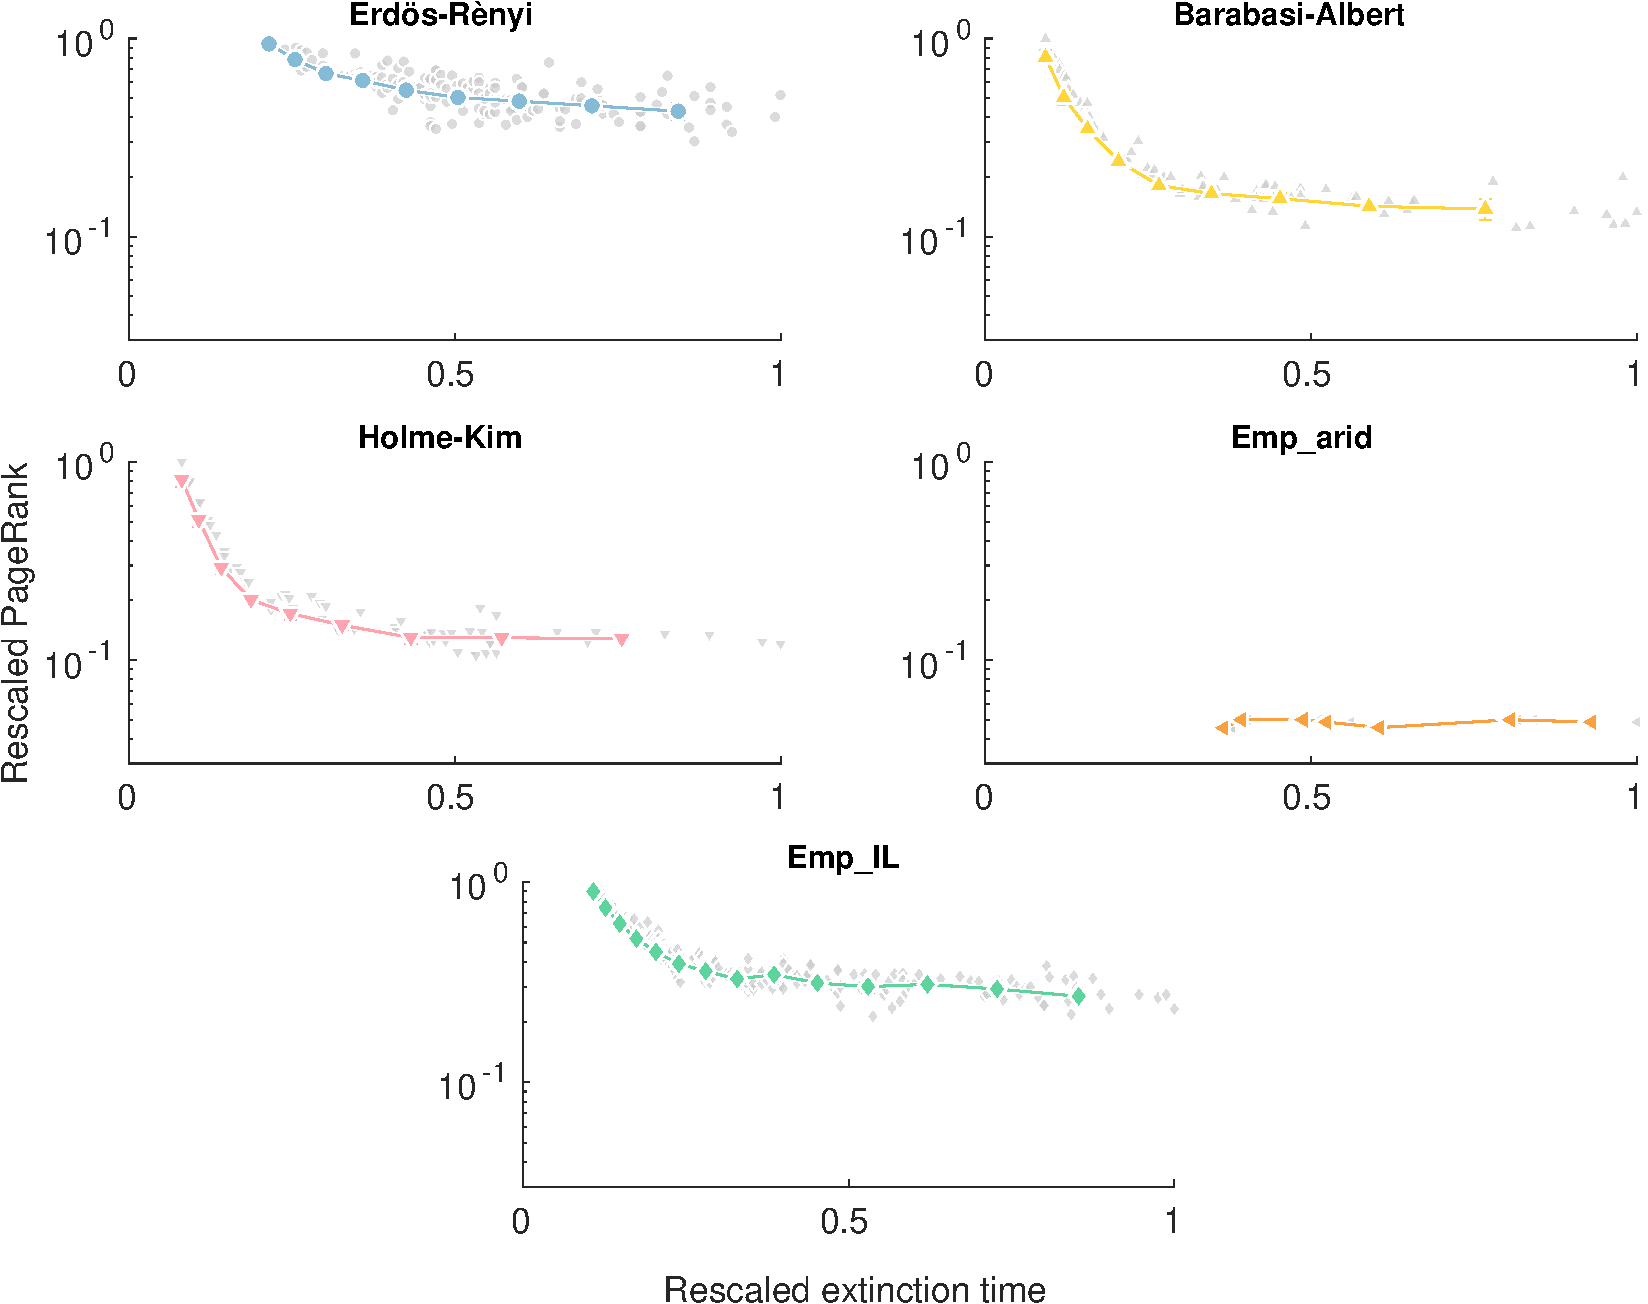
\includegraphics[width=\textwidth]{figures/chp2/figSI2_comp.pdf}
    \caption[Evolution of PageRank of extinct species]{PageRank in function of the time a species becomes extinct. These panels report the same data shown in Figure~\ref{chp2:fig:8}b. Each gray point is a species. Colored points are the mean PageRank calculated over logarithmically spaced bins. Error bars (sometimes too short to be seen) denote the standard deviation from the mean.}
    \label{chp2:fig:SI2_comp}
\end{figure}


